% CVPR 2025 Paper Template; see https://github.com/cvpr-org/author-kit

\documentclass[10pt,twocolumn,letterpaper]{article}

%%%%%%%%% PAPER TYPE  - PLEASE UPDATE FOR FINAL VERSION
% \usepackage{cvpr}              % To produce the CAMERA-READY version
% \usepackage[review]{cvpr}      % To produce the REVIEW version
\usepackage[pagenumbers]{cvpr} % To force page numbers, e.g. for an arXiv version

% Import additional packages in the preamble file, before hyperref
%
% --- inline annotations
%
\newcommand{\red}[1]{{\color{red}#1}}
\newcommand{\todo}[1]{{\color{red}#1}}
\newcommand{\TODO}[1]{\textbf{\color{red}[TODO: #1]}}
% --- disable by uncommenting  
% \renewcommand{\TODO}[1]{}
% \renewcommand{\todo}[1]{#1}

%%%%%%%%%%%
\usepackage{booktabs}
\usepackage{multirow}
\usepackage{adjustbox}
\usepackage{tabularx, colortbl}
\usepackage{bbding}
%\usepackage{hyperref}       % hyperlinks
\usepackage{url}            % simple URL typesetting
\usepackage{booktabs}       % professional-quality tables
\usepackage{amsfonts}       % blackboard math symbols
\usepackage{nicefrac}       % compact symbols for 1/2, etc.
\usepackage{microtype}      % microtypography
\usepackage{xcolor}         % colors
\usepackage{amsmath}
\usepackage{amssymb}
\usepackage{enumitem}
\usepackage{amsthm}

%%%%%%%%%%%
\newtheorem{theorem}{Theorem}
\newtheorem{lemma}{Lemma}
\newtheorem{assumption}{Assumption}
\newtheorem{proposition}{Proposition}

%%%%%%%%%%%
\DeclareMathOperator{\x}{\mathbf{x}}
\DeclareMathOperator{\Phix}{\mathbf{\Phi x}}
\DeclareMathOperator{\y}{\mathbf{y}}
\DeclareMathOperator{\PhiTy}{\mathbf{\Phi}^T \mathbf{y}}
\DeclareMathOperator{\PhiTu}{\mathbf{\Phi}^T \mathbf{u}}
\DeclareMathOperator{\bfPhi}{\mathbf{\Phi}}
\DeclareMathOperator{\bfA}{\mathbf{A}}
\DeclareMathOperator{\bfW}{\mathbf{W}}
\DeclareMathOperator{\R}{\mathbb{R}}
\DeclareMathOperator{\I}{\mathbf{I}}
\DeclareMathOperator{\zz}{\mathbf{z}}
\DeclareMathOperator{\rr}{\mathbf{r}}
\DeclareMathOperator{\bb}{\mathbf{b}}
\DeclareMathOperator{\bfs}{\mathbf{s}}
\DeclareMathOperator{\hh}{\mathbf{h}}
\DeclareMathOperator{\bfu}{\mathbf{u}}
\DeclareMathOperator{\barAlpha}{\bar{\alpha}}
\DeclareMathOperator{\bfd}{\mathbf{d}}


% It is strongly recommended to use hyperref, especially for the review version.
% hyperref with option pagebackref eases the reviewers' job.
% Please disable hyperref *only* if you encounter grave issues, 
% e.g. with the file validation for the camera-ready version.
%
% If you comment hyperref and then uncomment it, you should delete *.aux before re-running LaTeX.
% (Or just hit 'q' on the first LaTeX run, let it finish, and you should be clear).
\definecolor{cvprblue}{rgb}{0.21,0.49,0.74}
\usepackage[pagebackref,breaklinks,colorlinks,allcolors=cvprblue]{hyperref}

%%%%%%%%% PAPER ID  - PLEASE UPDATE
\def\paperID{83} % *** Enter the Paper ID here
\def\confName{CVPR}
\def\confYear{2025}

%%%%%%%%% TITLE
\title{One-Minute Video Generation with Test-Time Training}

%%%%%%%%% AUTHORS
\author{
\fontsize{10}{12}\selectfont
        Karan Dalal\thanks{Joint first authors}$^{*4} $
        \hspace{.1em} Daniel Koceja$^{*2}$\hspace{0.1em} Gashon Hussein$^{*2}$ \hspace{0.1em} Jiarui Xu$^{*1,3}$ 
        \hspace{0.1em} Yue Zhao\thanks{Joint second authors}$^{\dagger 5}$ \hspace{0.1em} Youjin Song$^{\dagger 2}$ \\[0.4em]
\fontsize{10}{12}\selectfont
        Shihao Han$^{1}$ \hspace{0.1em} Ka Chun Cheung$^{1}$ \hspace{0.1em} Jan Kautz$^{1}$ \hspace{0.1em} Carlos Guestrin$^{2}$ 
        \hspace{0.1em} Tatsunori Hashimoto$^{2}$ \hspace{0.1cm} Sanmi Koyejo$^{2}$ \\[0.4em]
\fontsize{10}{12}\selectfont
        Yejin Choi$^{1}$ \hspace{.1em} Yu Sun$^{1,2}$ \hspace{.1em} Xiaolong Wang$^{1,3}$ 
        \\[0.4em]
\fontsize{10}{12}\selectfont
        $^1$NVIDIA \quad
        $^2$Stanford University \quad
        $^3$UCSD \quad
        $^4$UC Berkeley \quad
        $^5$UT Austin
}

\begin{document}

\twocolumn[{
    \maketitle
    \centering
    \includegraphics[width=\textwidth]{figs/video.pdf}
    \captionof{figure}{TTT layers enable a pre-trained Diffusion Transformer to generate one-minute videos from text storyboards. 
    We use \textit{Tom and Jerry} cartoons as a proof of concept.
    The videos tell complex stories with coherent scenes composed of dynamic motion.
    Every video is produced directly by the model in a single shot, without editing, stitching, or post-processing. 
    Every story is newly created.
    }
    \label{fig:videos}
    \vspace{4ex}
}]

\footnotetext[1]{Joint first authors.~~$^\dagger$ Joint second authors.}
\footnotetext[0]{Accepted to The IEEE/CVF Conference on Computer Vision and Pattern Recognition (CVPR) 2025}


\begin{abstract}
\renewcommand{\thefootnote}{\fnsymbol{footnote}} 
    \footnotetext[1]{Equal contribution.}
\DefineFNsymbols*{1}{\Letter}
\setfnsymbol{1}

\renewcommand{\thefootnote}{\fnsymbol{footnote}} 
    \footnotetext[1]{Corresponding authors: Peng Li (lipeng@air.tsinghua.edu.cn) and Yang Liu (liuyang2011@tsinghua.edu.cn).}
\renewcommand{\thefootnote}{\arabic{footnote}}

Recently, model merging methods have demonstrated powerful strengths in combining abilities on various tasks from multiple Large Language Models (LLMs). While previous model merging methods mainly focus on merging homogeneous models with identical architecture, they meet challenges when dealing with Multimodal Large Language Models (MLLMs) with inherent heterogeneous property, including differences in model architecture and the asymmetry in the parameter space. In this work, we propose \ours\footnote{AdaMMS represents \textbf{Ada}ptive \textbf{M}apping, \textbf{M}erging, and \textbf{S}earching.}, a novel model merging method tailored for heterogeneous MLLMs. Our method tackles the challenges in three steps: mapping, merging and searching. Specifically, we first design mapping function between models to apply model merging on MLLMs with different architecture. Then we apply linear interpolation on model weights to actively adapt the asymmetry in the heterogeneous MLLMs. Finally in the hyper-parameter searching step, we propose an unsupervised hyper-parameter selection method for model merging. As the first model merging method capable of merging heterogeneous MLLMs without labeled data, extensive experiments on various model combinations demonstrated that \ours outperforms previous model merging methods on various vision-language benchmarks.\footnote{Code at \url{https://github.com/THUNLP-MT/AdaMMS}.}
% TODO: 再excited一点! proving that xxx, 或者是具体的数值提升,实在不行讲conclusion里边的unlock那件事情

% We hope this work unlocks the architectural constraints and alleviates the need for supervised requirements in model merging for MLLMs, facilitating the integration of diverse models into a cohesive system.

\end{abstract}

\section{Introduction}
\label{sec:intro}



Multimodality provides a rich signal for perceiving and understanding the world.
Advances in vision  
\citep{radford2021learning,oquab2023dinov2,zhai2023sigmoidsiglip,fini2024multimodalaimv2},
\edit{audio \citep{huang2022masked,elizalde2023clap,chen2022wavlm,hsu2021hubert}} 
and language models \citep{achiam2023gpt4,team2023gemini,dubey2024llama3}  
have enabled the development of powerful multimodal models that understand
language, images, and audio. A common approach involves grafting separately
pre-trained unimodal models, \edit{such as connecting a vision encoder to the input
layer of an
LLM~\citep{laurenccon2024mattersidefics2,shukor2023epalm,alayrac2022flamingo,
xue2024xgenblip3,beyer2024paligemma,wang2024qwen2,liu2024improvedllava,zhang2023videollama,kong2024audioflam,defossez2024moshi}.}


Although this seems like a convenient approach, it remains an open question
whether such late-fusion strategies are inherently optimal \edit{for
understanding multimodal signals}.  Moreover, with abundant multimodal data
available, initializing from unimodal pre-training is potentially detrimental,
as it may introduce biases that prevent the model from \edit{fully leveraging
cross-modality co-dependancies}.
An additional challenge is scaling such systems;  each component (e.g., vision
encoder, LLM) has its own set of hyperparameters, \edit{pre-training data
mixtues}, and \edit{scaling properties with respect to the amount} of data and
compute applied. A more flexible architecture might allow the model to
dynamically allocate its capacity across modalities, simplifying scaling
efforts.


In this work, we focus on the scaling properties of native multimodal models
trained from the ground up on multimodal data. We first investigate whether
\edit{the commonly adopted} late-fusion architectures hold an intrinsic
advantage by comparing them to early-fusion models, which process raw multimodal
inputs without relying on \edit{dedicated vision encoders}.  
We conduct scaling experiments on early and late fusion architectures, deriving
scaling laws to predict their performance and compute-optimal configurations.
Our findings indicate that late fusion offers no inherent advantage when
\edit{trained} from scratch. Instead, early-fusion models are more efficient and
are easier to scale. Furthermore, we observe that native multimodal models
follow scaling laws similar to those of LLMs~\citep{hoffmann2022training},
albeit with slight variations in scaling coefficients across modalities and
datasets. Our results suggest that model parameters and training tokens should
be scaled \edit{roughly equally} for optimal performance.
Moreover, we find that different \edit{multimodal} training mixtures exhibit
similar overall trends, indicating that our findings are likely to generalize to
a broader range of settings.


While our findings favor early fusion, multimodal data is inherently
heterogeneous, suggesting that some degree of parameter specialization may still
offer benefits. To \edit{investigate} this, we \edit{explore leveraging} Mixture
of Experts (MoEs)~\citep{shazeer2017outrageously}, a technique that enables the
model to dynamically allocate specialized parameters across modalities in a
symmetric and parallel manner, in contrast to late-fusion models, which are
asymmetric and process data sequentially. Training native multimodal models with
MoEs results in significantly improved performance and \edit{therefore,} faster
convergence. \edit{Our scaling laws for MoEs suggest that scaling number of
training tokens is more important the number of active parameters. This
unbalanced scaling is different from what is observed for dense models, due to
the higher number of total parameters for sparse models.} \edit{In addition,
}our analysis reveals that experts tend to specialize in different modalities,
with this specialization being particularly prominent in the early and last
layers. 





\begin{figure}[t!]
    \centering
    \captionsetup{type=figure}
    \begin{subfigure}[t]{0.48\linewidth}
        \begin{tikzpicture}[
    spy using outlines={rectangle, magnification=2, size=0.5in, connect spies} %
]
    \begin{axis}[
        legend pos=south west,
        grid=both,
        grid style={line width=.1pt, draw=gray!10},
        major grid style={line width=.2pt,draw=gray!50},
        minor tick num=2,
        axis x line*=bottom,
        axis y line*=left,
        xmode=log, %
        log basis x=10, %
        height=2.5in,
        width=1.1\linewidth,
        xtick distance=1e02,
        ylabel={\footnotesize{Validation Loss ($L$)}},
        ytick distance=0.5,
        yticklabel style={font=\footnotesize, /pgf/number format/fixed, /pgf/number format/precision=2},
        xlabel={\footnotesize{FLOPs ($C$)}},
        xticklabel style={font=\footnotesize},
        legend style={cells={align=left}, font=\footnotesize, fill opacity=0.7}, %
        mark options={solid},
    ]




    \addplot[line width=1.5pt, dashdotdotted, color=EarlyGradStart!50!EarlyGradEnd, samples=50, domain=5e18:5e23] {29.57440597247478*x^-0.04919003913934263};
    \addlegendentry{\scalebox{0.9}{Early: $L \propto C^{-0.0492}$}};
    \addplot[line width=1.5pt, dashdotdotted, color=LateGradStart!50!LateGradEnd, samples=50, domain=5e18:5e23] {30.038509408784137*x^-0.049424801983112776};
    \addlegendentry{\scalebox{0.9}{Late: $L \propto C^{-0.0494}$}};

    \addplot[line width=1.5pt, dashdotdotted, color=MOEGradStart!50!MOEGradEnd, samples=50, domain=5e18:5e23] {26.287135104499598*x^-0.04742807363789748};
    \addlegendentry{\scalebox{0.9}{MoE: $L \propto C^{-0.0474}$}};

    \begin{scope}
        \spy on (1.5,3.2) in node [right] at (3.8,3.5);
    \end{scope}

    \end{axis}
\end{tikzpicture}
    \end{subfigure}
    \hfill
    \begin{subfigure}[t]{0.48\linewidth}
        \begin{tikzpicture}
    \begin{axis}[
        legend pos=north west,
        grid=both,
        grid style={line width=.1pt, draw=gray!10},
        major grid style={line width=.2pt,draw=gray!50},
        minor tick num=2,
        axis x line*=bottom,
        axis y line*=left,
        xmode=log, %
        log basis x=10, %
        height=2.5in,
        width=1.1\linewidth,
        xtick distance=1e02,
        ylabel={\footnotesize{$N/D$}},
        ylabel style={yshift=-1ex},
        xlabel={\footnotesize{FLOPs ($C$)}},
        yticklabel style={font=\footnotesize},
        xticklabel style={font=\footnotesize},
        legend style={cells={align=left}, font=\footnotesize, fill opacity=0.7}, %
        mark options={solid},
    ]

    \addplot[line width=1.7pt, dashdotdotted, color=EarlyGradStart!50!EarlyGradEnd, samples=50, domain=5e18:5e23] {((780.3128750575453^-1)*x^(0.05302278709608001)};
    \addlegendentry{\scalebox{0.9}{Early: $\frac{N}{D} \propto C^{0.053}$}};
    \addplot[line width=1.7pt, dashdotdotted, color=LateGradStart!50!LateGradEnd, samples=50, domain=5e18:5e23] {(1880.7495777617235^-1)*x^(0.07616482680724829)};
    \addlegendentry{\scalebox{0.9}{Late: $\frac{N}{D} \propto C^{0.076}$}};

    \addplot[line width=1.7pt, dashdotdotted, color=MOEGradStart!50!MOEGradEnd, samples=50, domain=5e18:5e23] {((5.024013439838208e-05)^-1)*x^(-0.31205022008476146)};
    \addlegendentry{\scalebox{0.9}{MoE: $\frac{N}{D} \propto C^{-0.312}$}};

    \end{axis}
\end{tikzpicture}
    \end{subfigure}
    \vspace{-3mm}
    \caption{\textbf{Scaling properties of Native Multimodal Models.} Based on
    the scaling laws study in \cref{sec:scaling_laws_early}, we observe: (1)
    early and late fusion models provide on par validation loss $L$ when trained
    using the same compute budget $C$ (in FLOPs); (2) This performance is
    achieved via a different trade-off between parameters $N$ and number of
    training tokens $D$, where early-fusion models requires fewer parameters.
    \edit{; (3) Sparse early-fusion models achieve lower loss and require more
    training tokens for a given FLOP budget.} 
    }
    \label{fig:teaser}
\end{figure}


\subsection{Summary of our findings}
Our findings can be summarized as follows:

\cpar{Native early and late fusion perform on par:} \edit{Early fusion models trained
from scratch}
perform on par with their late-fusion counterparts, with a
slight advantage to early-fusion models for low compute budgets
(\cref{fig:early_vs_early_init_scaledata}). Furthermore, our scaling laws study
indicates that the compute-optimal models for early and late fusion perform
similarly as the compute budget increases~(\cref{fig:teaser} Left).

\cpar{NMMs scale similarly to LLMs:} The scaling laws of native multimodal
models follow similar laws as text-only LLMs with slightly varying  scaling
exponents depending on the target data type and training mixture
(\cref{tab:early_vs_late_coeffs}).

\cpar{Late-fusion requires more parameters:}
Compute-optimal late-fusion models require a higher parameters-to-data ratio
when compared to early-fusion (\cref{fig:teaser} Right).

\cpar{Sparsity significantly benefits early-fusion NMMs:} Sparse NMMs exhibit
significant improvements compared to their dense counterparts at the same
inference cost~(\cref{fig:dense_vs_moe_scaledata}). Furthermore, they implicitly
learn modality-specific weights when trained with
sparsity~(\cref{fig:app_moes_specialization}). \edit{In addition,
compute-optimal models rely more on scaling the number of training tokens than
the number of active parameters as the compute-budget grows (\cref{fig:teaser} Right).}

\cpar{Modality-agnostic routing beats Modality-aware routing for Sparse NMMs:}
Training sparse mixture of experts with modality-agnostic routing consistently
outperforms models with modality-aware routing
(\cref{fig:hard_vs_moe_scaledata}).


\vspace{-5pt}





\section{Test-Time Training Layers}
\label{sec:prelim}

Following standard practice~\cite{meta2024moviegen, yang2024cogvideox}, 
each video is pre-processed into a sequence of $T$ tokens, where $T$ is determined by its duration and resolution.
This section reviews Test-Time Training (TTT) layers for general sequence modeling, using some of the exposition in Section 2 of~\cite{sun2024ttt}.
We first discuss how to process general input sequences in a causal manner (chronological order).
Section~\ref{sec:method} discusses how to use RNN layers in a non-causal backbone by invoking them in opposite directions.

\subsection{TTT as Updating a Hidden State}
\label{subsec:hidden}
All RNN layers compress historical context in a hidden state of fixed size. This compression has two consequences.
On one hand, mapping an input token $x_t$ to output token $z_t$ is efficient, because both the update rule and output rule take constant time per token.
On the other hand, an RNN layer's ability to remember long context is limited by the amount of information its hidden state can store.
The goal of \cite{sun2024ttt} is to design RNN layers with expressive hidden states that can compress massive context.
As an inspiration, they observe that self-supervised learning can compress a massive training set into the weights of a machine learning model.

The key idea in \cite{sun2024ttt} is to use self-supervised learning to compress the historical context $x_1,\dots,x_t$ into a hidden state $W_t$, by making the context an unlabeled dataset and the hidden state the weights of a machine learning model $f$.
The update rule, illustrated in Figure~\ref{fig:ttt-layer}, is a step of gradient descent on some self-supervised loss $\ell$: 
\begin{equation}
\label{eq:update_naive}
W_t = W_{t-1} - \eta\,\nabla\ell(W_{t-1}; x_t),
\end{equation}
with learning rate $\eta$. Intuitively, the output token is just the prediction on $x_t$, made by $f$ with the updated weights $W_t$:
\begin{equation}
\label{eq:output_naive}
z_t = f(x_t; W_t).
\end{equation}

\noindent
One choice of $\ell$ is reconstructing $x_t$ itself. 
To make the learning problem nontrivial, one can first process $x_t$ into a corrupted input $\tilde{x}_t$ (see Subsection~\ref{subsec:task}), then optimize:
\begin{equation}    
\label{eq:recon}
\ell(W; x_t) = \| f(\tilde{x}_t; W) - x_t \|^2.
\end{equation}
Similar to denoising autoencoders~\citep{denoisingautoencoder}, $f$ needs to discover the correlations between dimensions of $x_t$ in order to reconstruct it from partial information $\tilde{x}_t$.

As with other RNN layers and self-attention, this algorithm that maps an input sequence $x_1,\dots,x_T$ to output sequence $z_1,\dots,z_T$ can be programmed into the forward pass of a sequence modeling layer.
Even at test time, the layer still trains a different sequence of weights $W_1, \dots, W_T$ for every input sequence. Therefore, it is called \emph{Test-Time Training (TTT) layer}.

Conceptually, calling backward on $\nabla\ell$ means taking gradients of gradients -- a well-explored technique in meta-learning.
TTT layers have the same interface as RNN layers and self-attention, therefore can be replaced in any larger network architecture. \cite{sun2024ttt} refers to training the larger network as the \emph{outer loop}, and training $W$ within each TTT layer as the \emph{inner loop}.

\subsection{Learning a Self-Supervised Task for TTT}
\label{subsec:task}
Arguably, the most important part of TTT is the self-supervised task specified by $\ell$. Instead of handcrafting a self-supervised task from human priors, \cite{sun2024ttt} takes a more end-to-end approach, learning it as part of the outer loop.
Starting from the naive reconstruction task in Equation~\ref{eq:recon}, they use a low-rank projection $\tilde{x}_t = \theta_Kx_t$, where $\theta_K$ is a matrix that is learnable in the outer loop.

Moreover, perhaps not all the information in $x_t$ is worth remembering, so the reconstruction label can also be a low-rank projection $\theta_Vx_t$ instead of $x_t$.
In summary, the self-supervised loss in \cite{sun2024ttt} is:
\begin{equation}
\label{eq:multi}
\ell(W; x_t) = \| f\left(\theta_K x_t; W\right) - \theta_V x_t \|^2.
\end{equation}
Lastly, since $\theta_Kx_t$ has fewer dimensions than $x_t$, \cite{sun2024ttt} can no longer use the output rule in Equation~\ref{eq:output_naive}.
So they make another projection $\theta_Qx_t$, and change the output rule to:
\begin{equation}
\label{eq:output}
z_t = f\left(\theta_Qx_t; W_t\right).
\end{equation}
Note that in the inner loop, only $W$ is optimized, therefore written as an argument of $\ell$; the $\theta$s are ``hyper-parameters" of this inner-loop loss function.
$\theta_K,\theta_V,\theta_Q$ are optimized in the outer loop, analogous to the Query, Key, and Value parameters of self-attention.

\subsection{TTT-MLP Instantiation}
Following \cite{sun2024ttt}, we instantiate the inner-loop model $f$ as a wrapper around $f_{\,\texttt{MLP}}$: a two-layer MLP similar to those in Transformers.
Specifically, the hidden dimension is $4 \times$ the input dimension, followed by a GELU activation~\cite{hendrycks2016gaussian}.
For better stability during TTT, $f$ always contains a Layer Norm and residual connection. That is,
$$f(x) = x + \texttt{LN}(f_{\,\texttt{MLP}}(x)).$$
A TTT layer with this $f$ is called TTT-MLP, which is the default instantiation throughout this paper.
In Section~\ref{sec:experiment} we also instantiate TTT-Linear (the $f$ above wrapping around a linear model) as a baseline.
\section{Method}
\label{sec:method}
Our approach, in line with previous methods, builds upon a pre-trained VLM, CLIP \cite{clip}. In this section, we detail the construction of our MMRL framework and the implementation specifics.

\subsection{Preliminary}
We begin by defining the notations used in our approach. CLIP comprises two encoders: an image encoder $\mathcal{V}$ and a text encoder $\mathcal{W}$.

\noindent \textbf{Image Encoding:} The image encoder $\mathcal{V}$ consists of $L$ transformer \cite{transformer} layers, denoted $\{\mathcal{V}_i\}_{i=1}^{L}$. Given an input image \( x \in \mathbb{R}^{H \times W \times 3} \), it is divided into \( M \) fixed-size patches, each projected into a patch embedding, resulting in \( E_0 \in \mathbb{R}^{M \times d_v} \), where $M$ represents the number of patches and $d_v$ the embedding dimension. The initial patch embeddings $E_0$ are combined with a learnable class token $c_0$ and positional encodings, forming the input sequence for the transformer layers. Each layer processes this sequence as
\begin{equation}
    [c_i, E_i] = \mathcal{V}_i([c_{i-1}, E_{i-1}]) \quad
    i = 1, 2, \ldots, L
    \nonumber
\end{equation}
After passing through all transformer layers, a patch projection layer, $P_v^c$, projects the output of the class token, $c_L$, into a shared V-L latent space,
\begin{equation}
    f = P_v^c(c_L)
    \nonumber
\end{equation}
where $f \in \mathbb{R}^{d}$.

\noindent \textbf{Text Encoding:} For an input text, \eg, ``A photo of a [CLASS].", it is tokenized and converted into embeddings $T_0 \in \mathbb{R}^{N \times d_t}$, where $N$ is the token length and $d_t$ the embedding dimension. Beginning-of-text (BOT) and end-of-text (EOT) tokens, denoted $b_0$ and $e_0$, mark the sequence boundaries. These token embeddings, with positional encodings, are passed through the text encoder's $L$ transformer layers, $\{\mathcal{W}_i\}_{i=1}^{L}$, as follows,
\begin{equation} 
    [b_i, T_i, e_i] = \mathcal{W}_i([b_{i-1}, T_{i-1}, e_{i-1}]) \quad i = 1, \ldots, L 
    \nonumber
\end{equation} 
After the final layer, the output of the EOT token, $e_L$, is projected into the shared V-L space using $P_t$,
\begin{equation} 
    w = P_{t}(e_{L}) \nonumber
\end{equation} 
where $w \in \mathbb{R}^{d}$.

\noindent \textbf{Classification with CLIP:} With the image feature $f$ and text features $\{w_c\}_{c=1}^C$ for $C$ classes, CLIP calculates the cosine similarity between $f$ and each $w_c$,
\begin{equation} 
    \text{sim}(f, w_c) = \frac{f \cdot w_c}{|f| |w_c|}, \nonumber 
\end{equation} 
where $|\cdot|$ represents the $L_2$ norm. Class probabilities are then computed using the softmax function,
\begin{equation} 
    p(y = c \mid f) = \frac{\exp(\text{sim}(f, w_c) / \tau)}{\sum_{i=1}^{C} \exp(\text{sim}(f, w_i) / \tau)} \nonumber 
\end{equation} 
where $\tau$ is a temperature parameter. The final predicted class is selected as the one with the highest probability score.

% The predicted class $\hat{y}$ is determined by: \begin{equation} 
%     \hat{y} = \arg\max_{c} , p(y = c \mid f). \nonumber
% \end{equation}


%-------------------------------------------------------------------------
\begin{figure*}[tb]
\setlength{\abovecaptionskip}{0.2cm}   %调整图片标题与图距离
\setlength{\belowcaptionskip}{-0.4cm}   %调整图片标题与下文距离
\centering
\setlength{\belowcaptionskip}{-0.39cm}   %调整图片标题与下文距离
  \includegraphics[width=0.7\linewidth]{fig/frame2.pdf}
  \caption{MMRL inference process, where different tasks utilize distinct features.}
  \label{framework2}
\end{figure*}
%-------------------------------------------------------------------------


\subsection{Multi-Modal Representation Learning (MMRL)} Our proposed MMRL aims to address the challenges of adapting pre-trained VLMs using few-shot data while maintaining generalization to new tasks. The training and inference frameworks of MMRL are shown in \cref{framework1} and \cref{framework2}, respectively. In the following, we describe the specifics of the methodology.


\subsubsection{Learnable Representation Space}
MMRL establishes a shared, learnable representation space $\mathcal{R}$ to facilitate multimodal interactions, initialized through sampling from a Gaussian distribution. Using a learnable mapping function $\mathcal{F}(\cdot)$, implemented as a linear layer, we project the tokens $R \in \mathbb{R}^{K \times d_r}$ in this space—where $K$ is the number of tokens and $d_r$ is the dimension of the representation space—into both visual and textual modalities,
\begin{align}
    R^v = \{R_i^v\}_{i=J-1}^{L-1} \quad & R_i^v = \mathcal{F}_i^v(R) \nonumber \\ 
    R^t = \{R_i^t\}_{i=J-1}^{L-1} \quad & R_i^t = \mathcal{F}_i^t(R) \nonumber 
\end{align}
where $R_i^v \in \mathbb{R}^{K \times d_v}$ and $R_i^t \in \mathbb{R}^{K \times d_t}$ represent the representation tokens for visual and textual modalities, respectively, in the $(i+1)$-th transformer layer. The index $J$ indicates the starting layer from which these representation tokens are integrated into the encoders.


\subsubsection{Integration into Higher Encoder Layers}
To preserve the generalized knowledge in the lower layers of the pre-trained CLIP model, the representation tokens $\mathcal{R}^v$ and $\mathcal{R}^t$ are integrated into the higher layers of the image encoder $\mathcal{V}$ and the text encoder $\mathcal{W}$, beginning from the $J$-th layer.


For the image encoder $\mathcal{V}$,
\begin{align}
    [c_i, E_i] &= \mathcal{V}_i([c_{i-1}, E_{i-1}]) \quad i = 1, \ldots, J-1 \nonumber \\  
    [c_i, \_, E_i] &= \mathcal{V}_i([c_{i-1}, R_{i-1}^v, E_{i-1}]) \quad i = J, \ldots, L - 1 \nonumber \\
    [c_i, R_i^v, E_i] &= \mathcal{V}_i([c_{i-1}, R_{i-1}^v, E_{i-1}]) \quad i = L \nonumber
\end{align}

For the text encoder $\mathcal{W}$, while previous prompt learning \cite{maple} involves replacing parts of $T_i$ to incorporate deep prompts, we retain the entire $T_i$ and insert $R_i^t$ before it, aiming to preserve the original textual information,
\begin{align}
    [b_i, T_i, e_i] &= \mathcal{W}_i([b_{i-1}, T_{i-1}, e_{i-1}]) \quad i = 1, \ldots, J-1 \nonumber \\  
    [b_i, \_, T_i, e_i] &= \mathcal{W}_i([b_{i-1}, R_{i-1}^t, T_{i-1}, e_{i-1}]) \nonumber \\
    &\hspace{4cm} i = J, \ldots, L-1 \nonumber \\
    [b_i, R_i^t, T_i, e_i] &= \mathcal{W}_i([b_{i-1}, R_{i-1}^t, T_{i-1}, e_{i-1}]) \quad i = L \nonumber
\end{align}
Note that due to the autoregressive nature of the text encoder, we adjust the attention mask matrix to accommodate the increased embedding length.


\subsubsection{Representation Learning}
Representation learning is designed to leverage representation tokens for dataset-specific adaptation, while the class token preserves the pre-trained knowledge of the original CLIP. Through a set of strategies aimed at retaining generalization during both training and inference, MMRL enables flexible inference for different tasks, as detailed below.


\begin{itemize} 

\item \textbf{Training Phase:} We optimize the features of both the representation tokens and the original class token, with the primary focus on representation features to preserve pre-trained knowledge. Specifically, the projection layer for the representation tokens is trainable, while that for the class token remains fixed. For the image encoder $\mathcal{V}$, after passing through $L$ transformer layers, we obtain the output $c_L \in \mathbb{R}^{d_v}$ for the class token and $R_L^v \in \mathbb{R}^{K \times d_v}$ for the $K$ representation tokens. The final output of the representation tokens, $r_L$, is derived by averaging across the $K$ tokens,
\begin{equation}
    r_L = \text{Mean}(R_L^v) \nonumber
\end{equation}
where $r_L \in \mathbb{R}^{d_v}$. We then apply the patch projection layers to map the outputs of both the class and representation tokens into the common V-L latent space, yielding the class features $f_c$ and representation features $f_r$.
\begin{equation}
    f_c = P_v^c(c_L) \quad f_r = P_v^r(r_L) \nonumber
\end{equation}
Here, $P_v^c$ is the original, frozen patch projection layer of CLIP for class features, while $P_v^r$ for representation features is trainable.

For the text encoder $\mathcal{W}$, following the sequential nature of text, we map the EOT token $e_L$—as in the original CLIP model—after processing through $L$ transformer layers into the common V-L space, yielding the text features.
\begin{equation} 
    w = P_{t}(e_{L}) \nonumber
\end{equation}
With the image features $f_c$, $f_r$, and the text classifiers $\{w_c\}_{c=1}^C$ for $C$ classes, we apply cross-entropy loss to separately optimize the class and representation features,
\begin{align}
\setlength\abovedisplayskip{3pt}
\setlength\belowdisplayskip{3pt}
    \mathcal{L}_{ce}^c &= -\sum_c^C y_c \log p(y = c \mid f_c) \nonumber \\
    \mathcal{L}_{ce}^r &= -\sum_c^C y_c \log p(y = c \mid f_r) \nonumber
\end{align}
where $y_c = 1$ if the image $x$ belongs to class $c$, and $y_c = 0$ otherwise. To further preserve the generalization of class features, we maximize the cosine similarity between $(f_c, w)$ and the frozen CLIP features $(f_0, w_0)$, explicitly guiding the training trajectory,
\begin{equation}
    \mathcal{L}_{cos}^v = 1 - \frac{f_c \cdot f_0}{|f_c| |f_0|} \quad \mathcal{L}_{cos}^t = 1 - \frac{1}{C}\sum_c^C \frac{w^c \cdot w_0^c}{|w^c| |w_0^c|}, \nonumber
\end{equation}
The final MMRL loss function is
\begin{equation}
    \mathcal{L}_{MMRL} = \alpha \mathcal{L}_{ce}^c + (1 - \alpha) \mathcal{L}_{ce}^r + \lambda (\mathcal{L}_{cos}^v + \mathcal{L}_{cos}^t)  \nonumber
\end{equation}
where $\alpha$ controls the balance between the features, and $\lambda$ is the penalty coefficient.

\item \textbf{Testing on Base Classes:} 
For in-distribution classes seen during training, we combine the dataset-specific representation features with the class features that preserve generalizability. The probability of an in-distribution test sample $x$ belonging to the $c$-th class is
\begin{equation}
    p(y = c \mid x) = \alpha \cdot p(y = c \mid f_c) + (1-\alpha) \cdot p(y = c \mid f_r) \nonumber
\end{equation}
where $f_c$ and $f_r$ are features extracted from the class token and representation tokens, respectively.

\item  \textbf{Testing on Novel Classes:}
For classes unseen during training or for new datasets, we rely solely on the class tokens, which retain generalized knowledge.
\begin{equation}
    p(y = c \mid x) = p(y = c \mid f_c) \nonumber
\end{equation}
\end{itemize}



% Then the predicted class $\hat{y}$ is determined by, 
% \begin{equation} 
%     \hat{y} = \arg\max_{c} , p(y = c \mid x). \nonumber
% \end{equation}



\begin{table*}[t]
\centering
\setlength{\abovecaptionskip}{0.15cm}   %调整表格标题与表格距离
\caption{Comparison of MMRL with previous state-of-the-art methods on base-to-novel generalization across 11 datasets. Bold values indicate the best results. MMRL consistently enhances base class performance without compromising generalization.}
\label{base_to_novel}
\renewcommand\arraystretch{1.06}
\setlength{\tabcolsep}{2.87mm}{
\resizebox{0.85\textwidth}{!}{
    \begin{tabular}{@{}r|ccc|ccc|ccc|ccc@{}}
    \toprule
    \multirow{2}{*}{Method} &
      \multicolumn{3}{c|}{Average} &
      \multicolumn{3}{c|}{ImageNet} &
      \multicolumn{3}{c|}{Caltech101} &
      \multicolumn{3}{c}{OxfordPets} \\
     &
      Base &
      Novel &
      HM &
      Base &
      Novel &
      HM &
      Base &
      Novel &
      HM &
      Base &
      Novel &
      HM \\ \midrule
    $\text{CLIP}_{\text{ (ICML2021)}}$ &
      69.34 &
      74.22 &
      71.70 &
      72.43 &
      68.14 &
      70.22 &
      96.84 &
      94.00 &
      95.40 &
      91.17 &
      97.26 &
      94.12 \\
    $\text{CoOp}_{\text{ (IJCV2022)}}$ &
      82.69 &
      63.22 &
      71.66 &
      76.47 &
      67.88 &
      71.92 &
      98.00 &
      89.81 &
      93.73 &
      93.67 &
      95.29 &
      94.47 \\
    $\text{CoOpOp}_{\text{ (CVPR2022)}}$ &
      80.47 &
      71.69 &
      75.83 &
      75.98 &
      70.43 &
      73.10 &
      97.96 &
      93.81 &
      95.84 &
      95.20 &
      97.69 &
      96.43 \\
    $\text{ProDA}_{\text{ (CVPR2022)}}$ &
      81.56 &
      72.30 &
      76.65 &
      75.40 &
      70.23 &
      72.72 &
      98.27 &
      93.23 &
      95.68 &
      95.43 &
      97.83 &
      96.62 \\
    $\text{KgCoOp}_{\text{ (CVPR2023)}}$ &
      80.73 &
      73.60 &
      77.00 &
      75.83 &
      69.96 &
      72.78 &
      97.72 &
      94.39 &
      96.03 &
      94.65 &
      97.76 &
      96.18 \\
    $\text{MaPLe}_{\text{ (CVPR2023)}}$ &
      82.28 &
      75.14 &
      78.55 &
      76.66 &
      70.54 &
      73.47 &
      97.74 &
      94.36 &
      96.02 &
      95.43 &
      97.76 &
      96.58 \\
    $\text{PromptSRC}_{\text{ (ICCV2023)}}$ &
      84.26 &
      76.10 &
      79.97 &
      77.60 &
      70.73 &
      74.01 &
      98.10 &
      94.03 &
      96.02 &
      95.33 &
      97.30 &
      96.30 \\
    $\text{ProVP}_{\text{ (IJCV2024)}}$ &
      85.20 &
      73.22 &
      78.76 &
      75.82 &
      69.21 &
      72.36 &
      98.92 &
      94.21 &
      96.51 &
      95.87 &
      97.65 &
      \textbf{96.75} \\
    $\text{MetaPrompt}_{\text{ (TIP2024)}}$ &
      83.65 &
      75.48 &
      79.09 &
      77.52 &
      70.83 &
      74.02 &
      98.13 &
      94.58 &
      96.32 &
      95.53 &
      97.00 &
      96.26 \\
    $\text{TCP}_{\text{ (CVPR2024)}}$ &
      84.13 &
      75.36 &
      79.51 &
      77.27 &
      69.87 &
      73.38 &
      98.23 &
      \textbf{94.67} &
      96.42 &
      94.67 &
      97.20 &
      95.92 \\
    $\text{MMA}_{\text{ (CVPR2024)}}$ &
      83.20 &
      76.80 &
      79.87 &
      77.31 &
      71.00 &
      74.02 &
      98.40 &
      94.00 &
      96.15 &
      95.40 &
      \textbf{98.07} &
      96.72 \\ \midrule
    $\text{MMRL}_{\text{ (Ours)}}$ &
      \textbf{85.68} &
      \textbf{77.16} &
      \textbf{81.20} &
      \textbf{77.90} &
      \textbf{71.30} &
      \textbf{74.45} &
      \textbf{98.97} &
      94.50 &
      \textbf{96.68} &
      \textbf{95.90} &
      97.60 &
      96.74 \\ \midrule \midrule
    \multirow{2}{*}{Method} &
      \multicolumn{3}{c|}{StanfordCars} &
      \multicolumn{3}{c|}{Flowers102} &
      \multicolumn{3}{c|}{Food101} &
      \multicolumn{3}{c}{FGVCAircraft} \\
     &
      Base &
      Novel &
      HM &
      Base &
      Novel &
      HM &
      Base &
      Novel &
      HM &
      Base &
      Novel &
      HM \\ \midrule
    $\text{CLIP}_{\text{ (ICML2021)}}$ &
      63.37 &
      74.89 &
      68.65 &
      72.08 &
      77.80 &
      74.83 &
      90.10 &
      91.22 &
      90.66 &
      27.19 &
      36.29 &
      31.09 \\
    $\text{CoOp}_{\text{ (IJCV2022)}}$ &
      78.12 &
      60.40 &
      68.13 &
      97.60 &
      59.67 &
      74.06 &
      88.33 &
      82.26 &
      85.19 &
      40.44 &
      22.30 &
      28.75 \\
    $\text{CoOpOp}_{\text{ (CVPR2022)}}$ &
      70.49 &
      73.59 &
      72.01 &
      94.87 &
      71.75 &
      81.71 &
      90.70 &
      91.29 &
      90.99 &
      33.41 &
      23.71 &
      27.74 \\
    $\text{ProDA}_{\text{ (CVPR2022)}}$ &
      74.70 &
      71.20 &
      72.91 &
      97.70 &
      68.68 &
      80.66 &
      90.30 &
      88.57 &
      89.43 &
      36.90 &
      34.13 &
      35.46 \\
    $\text{KgCoOp}_{\text{ (CVPR2023)}}$ &
      71.76 &
      75.04 &
      73.36 &
      95.00 &
      74.73 &
      83.65 &
      90.50 &
      91.70 &
      91.09 &
      36.21 &
      33.55 &
      34.83 \\
    $\text{MaPLe}_{\text{ (CVPR2023)}}$ &
      72.94 &
      74.00 &
      73.47 &
      95.92 &
      72.46 &
      82.56 &
      90.71 &
      \textbf{92.05} &
      \textbf{91.38} &
      37.44 &
      35.61 &
      36.50 \\
    $\text{PromptSRC}_{\text{ (ICCV2023)}}$ &
      78.27 &
      74.97 &
      76.58 &
      98.07 &
      76.50 &
      85.95 &
      90.67 &
      91.53 &
      91.10 &
      42.73 &
      \textbf{37.87} &
      40.15 \\
    $\text{ProVP}_{\text{ (IJCV2024)}}$ &
      80.43 &
      67.96 &
      73.67 &
      98.42 &
      72.06 &
      83.20 &
      90.32 &
      90.91 &
      90.61 &
      \textbf{47.08} &
      29.87 &
      36.55 \\
    $\text{MetaPrompt}_{\text{ (TIP2024)}}$ &
      76.34 &
      75.01 &
      75.48 &
      97.66 &
      74.49 &
      84.52 &
      \textbf{90.74} &
      91.85 &
      91.29 &
      40.14 &
      36.51 &
      38.24 \\
    $\text{TCP}_{\text{ (CVPR2024)}}$ &
      80.80 &
      74.13 &
      77.32 &
      97.73 &
      75.57 &
      85.23 &
      90.57 &
      91.37 &
      90.97 &
      41.97 &
      34.43 &
      37.83 \\
    $\text{MMA}_{\text{ (CVPR2024)}}$ &
      78.50 &
      73.10 &
      75.70 &
      97.77 &
      75.93 &
      85.48 &
      90.13 &
      91.30 &
      90.71 &
      40.57 &
      36.33 &
      38.33 \\ \midrule
    $\text{MMRL}_{\text{ (Ours)}}$ &
      \textbf{81.30} &
      \textbf{75.07} &
      \textbf{78.06} &
      \textbf{98.97} &
      \textbf{77.27} &
      \textbf{86.78} &
      90.57 &
      91.50 &
      91.03 &
      46.30 &
      37.03 &
      \textbf{41.15} \\ \midrule \midrule
    \multirow{2}{*}{Method} &
      \multicolumn{3}{c|}{SUN397} &
      \multicolumn{3}{c|}{DTD} &
      \multicolumn{3}{c|}{EuroSAT} &
      \multicolumn{3}{c}{UCF101} \\
     &
      Base &
      Novel &
      HM &
      Base &
      Novel &
      HM &
      Base &
      Novel &
      HM &
      Base &
      Novel &
      HM \\ \midrule
    $\text{CLIP}_{\text{ (ICML2021)}}$ &
      69.36 &
      75.35 &
      72.23 &
      53.24 &
      59.90 &
      56.37 &
      56.48 &
      64.05 &
      60.03 &
      70.53 &
      77.50 &
      73.85 \\
    $\text{CoOp}_{\text{ (IJCV2022)}}$ &
      80.60 &
      65.89 &
      72.51 &
      79.44 &
      41.18 &
      54.24 &
      92.19 &
      54.74 &
      68.69 &
      84.69 &
      56.05 &
      67.46 \\
    $\text{CoOpOp}_{\text{ (CVPR2022)}}$ &
      79.74 &
      76.86 &
      78.27 &
      77.01 &
      56.00 &
      64.85 &
      87.49 &
      60.04 &
      71.21 &
      82.33 &
      73.45 &
      77.64 \\
    $\text{ProDA}_{\text{ (CVPR2022)}}$ &
      78.67 &
      76.93 &
      77.79 &
      80.67 &
      56.48 &
      66.44 &
      83.90 &
      66.00 &
      73.88 &
      85.23 &
      71.97 &
      78.04 \\
    $\text{KgCoOp}_{\text{ (CVPR2023)}}$ &
      80.29 &
      76.53 &
      78.36 &
      77.55 &
      54.99 &
      64.35 &
      85.64 &
      64.34 &
      73.48 &
      82.89 &
      76.67 &
      79.65 \\
    $\text{MaPLe}_{\text{ (CVPR2023)}}$ &
      80.82 &
      78.70 &
      79.75 &
      80.36 &
      59.18 &
      68.16 &
      94.07 &
      73.23 &
      82.35 &
      83.00 &
      78.66 &
      80.77 \\
    $\text{PromptSRC}_{\text{ (ICCV2023)}}$ &
      82.67 &
      78.47 &
      80.52 &
      83.37 &
      62.97 &
      71.75 &
      92.90 &
      73.90 &
      82.32 &
      87.10 &
      78.80 &
      82.74 \\
    $\text{ProVP}_{\text{ (IJCV2024)}}$ &
      80.67 &
      76.11 &
      78.32 &
      83.95 &
      59.06 &
      69.34 &
      \textbf{97.12} &
      72.91 &
      83.29 &
      \textbf{88.56} &
      75.55 &
      81.54 \\
    $\text{MetaPrompt}_{\text{ (TIP2024)}}$ &
      82.26 &
      79.04 &
      80.62 &
      83.10 &
      58.05 &
      68.35 &
      93.53 &
      75.21 &
      83.38 &
      85.33 &
      77.72 &
      81.35 \\
    $\text{TCP}_{\text{ (CVPR2024)}}$ &
      82.63 &
      78.20 &
      80.35 &
      82.77 &
      58.07 &
      68.25 &
      91.63 &
      74.73 &
      82.32 &
      87.13 &
      \textbf{80.77} &
      83.83 \\
    $\text{MMA}_{\text{ (CVPR2024)}}$ &
      82.27 &
      78.57 &
      80.38 &
      83.20 &
      \textbf{65.63} &
      73.38 &
      85.46 &
      \textbf{82.34} &
      83.87 &
      86.23 &
      80.03 &
      82.20 \\ \midrule
    $\text{MMRL}_{\text{ (Ours)}}$ &
      \textbf{83.20} &
      \textbf{79.30} &
      \textbf{81.20} &
      \textbf{85.67} &
      65.00 &
      \textbf{73.82} &
      95.60 &
      80.17 &
      \textbf{87.21} &
      88.10 &
      80.07 &
      \textbf{83.89} \\ \bottomrule
    \end{tabular}
            }
}
\vspace{-0.3cm}
\end{table*}





\section{Evaluation}
\label{sec:experiment}

We perform human evaluation on a multi-axis benchmark for TTT-MLP and five baselines, all with linear complexity: local attention, TTT-Linear, Mamba 2, Gated DeltaNet, and sliding window attention layers.

\subsection{Baselines}
Except for local attention, all baselines are added to the same pre-trained CogVideo-X 5B using the approach in Subection~\ref{subsec:arch}; 
their modified architectures all have 7.2B parameters.
All baselines use the same fine-tuning recipe in Subsection~\ref{subsec:dataset}
and Appendix \ref{sec:appendix:implementation}.
Next we discuss the baselines in detail.
\vspace{0.2em}
\begin{itemize}[itemsep=0.2em]
\item\textbf{Local attention}: No modification to the original architecture, which performs self-attention on each 3-second segment independently.
\item\textbf{TTT-Linear}~\cite{sun2024ttt}: A TTT layer that instantiates $f(x) = x + \texttt{LN}(f_{\,\texttt{Linear}}(x))$, where $f_{\,\texttt{Linear}}$ is a linear model. 
\item\textbf{Mamba 2}~\cite{dao2024mamba2}: A modern RNN layer with a matrix hidden state, which is \(\approx4\times\) larger than the hidden state in TTT-Linear but \(\approx2\times\) smaller than that in TTT-MLP.
\item\textbf{Gated DeltaNet}~\cite{yang2025gateddeltanetworksimproving}: An extension of DeltaNet~\cite{yang2024parallelizing} and Mamba~2 with an improved update rule.
\item\textbf{Sliding-window attention}~\cite{beltagy2020longformerlongdocumenttransformer}: Self-attention with a fixed window of $8192$ tokens (about 1.5 seconds of video). 
% Since CogVideo-X has 42 attention layers, their receptive field covers the entire one-minute context length.
\end{itemize}

\subsection{Evaluation Axes and Protocol}
\label{subsec:quan_eval}
From the six evaluation axes in MovieGen~\cite{meta2024moviegen}, we adopt the four relevant to our domain for human evaluation.\footnote{
Out of the six axes in MovieGen, we omit ``realness" which does not apply to cartoons.
We also omit ``motion completeness" which ``measures whether the output video contains enough motion", because all videos in our domain have highly dynamic motion.
We adapt ``frame consistency" to ``temporal consistency" to also include consistency across scenes.}

\begin{landscape}
\begin{figure}
    \centering
    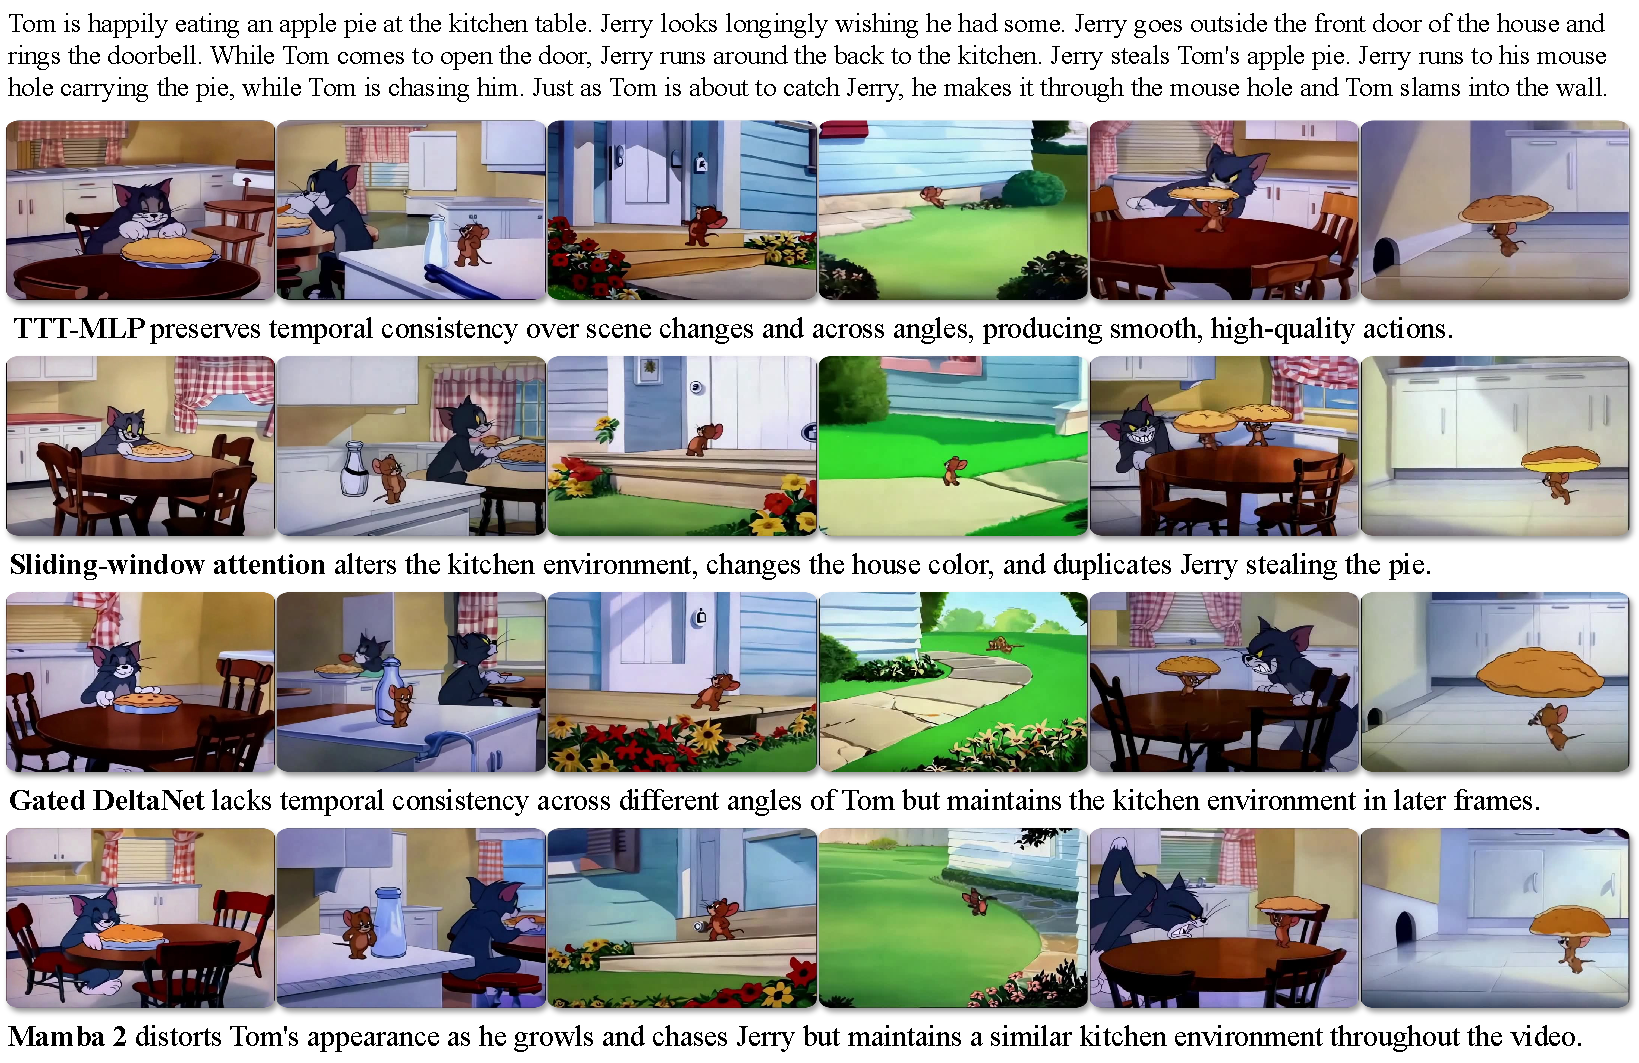
\includegraphics[width=1.28\textwidth]{figs/qualitative.pdf}
    \caption{Video frames comparing TTT-MLP against Gated DeltaNet and sliding-window attention, the leading baselines in our human evaluation. 
    TTT-MLP demonstrates better scene consistency by preserving details across transitions and better motion naturalness by accurately depicting complex actions.}
    \label{fig:qualitative}
\end{figure}
\end{landscape}

\twocolumn[{
\centering
\setlength{\tabcolsep}{6pt}
\renewcommand{\arraystretch}{1.3}
\begin{tabular}{lcccc|c}
    \toprule
     & Text following & Motion naturalness & Aesthetics & Temporal consistency & Average \\
    \midrule
    {Mamba 2} & 985 & 976 & 963 & 988 & 978  \\
    {Gated DeltaNet} & 983 & 984 & 993 & 1004 & 991 \\
    {Sliding window} & \textbf{1016} & 1000 & 1006 & 975 & 999 \\
    {TTT-MLP} & 1014 & \textbf{1039} & \textbf{1037} & \textbf{1042} & \textbf{1033} \\
    \bottomrule
    \end{tabular}
    \captionof{table}{Human evaluation results for one-minute videos. TTT-MLP improves over the second best method by 34 Elo points on average. 
    Axes with the most improvements are scene consistency (+38) and motion smoothness (+39). For context, GPT-4 scores 46 Elo points over GPT-3.5 Turbo, and GPT-4o scores 29 over GPT-4 Turbo in Chatbot Arena~\cite{chiang2024chatbot}.}
    \label{tab:multiaxis_evaluation}

    \begin{minipage}[c]{0.66\textwidth}
    \vspace{2ex}
        \includegraphics[width=\linewidth]{figs/latency.pdf}
    \end{minipage}\hfill
    \begin{minipage}[c]{0.33\textwidth}
    \vspace{2ex}
        \captionof{figure}{
        For 63-second videos, inference with full attention (over 300k tokens) would have taken $11\times$ longer than local attention, and training $12\times$ longer, as discussed in Section~\ref{sec:intro}.
        TTT-MLP takes $2.5\times$ and $3.8\times$ respectively -- significantly more efficient than full attention, but still less efficient than, for example, Gated DeltaNet, which takes $1.8\times$ longer than local attention in both inference and training.
        }
        \label{fig:your_label}
    \end{minipage}
    \vspace{1.0em}
}]

\begin{itemize}[itemsep=0.2em]
\item \textbf{Text following}: ``aligment with the provided prompt."
\item \textbf{Motion naturalness}: ``natural limb
movements, facial expressions, and adherence to physical laws.
Motion that appears unnatural or uncanny will be penalized."
\item \textbf{Aesthetics}: ``interesting and compelling content, lighting, color, and camera effects."
\item \textbf{Temporal consistency}: both inside and across scenes.
\end{itemize}
The quoted descriptions are from MovieGen~\cite{meta2024moviegen}.


Our evaluation is based on pairwise preferences in blind comparisons, because directly rating long videos or ranking many of them at once is challenging.
Specifically, an evaluator is given a random axis from the four above and a random pair of videos sharing the same plot, then asked to indicate the better video for that axis.
To collect the pool of videos, we first sample 100 plots using Claude 3.7 Sonnet (in Format $1\rightarrow2\rightarrow3$ as discussed in Subsection~\ref{subsec:pipeline}), then generate one video per method per plot.
The methods generating the videos are always unknown to the evaluators.

Our evaluators were recruited on \texttt{prolific.com} with the filters: living in the U.S., English as a first language, aged 18 to 35 years, with at least 100 previous submissions and an approval rate of at least 98\%.
The demographics of our evaluators, disclosed on the website, are as follows.
\vspace{0.2em}
\begin{itemize}[itemsep=0.2em]
\item \textbf{Gender}: 50.78\% male, 47.66\% female, 1.56\% other.
\item \textbf{Ethnicity}: 57.03\% White, 23.44\% Black, 10.94\% Mixed, 5.47\% Asian, and 3.12\% other. 
\end{itemize}
Based on this information, we believe that our evaluators constitute a representative sample of the U.S. population.

\begin{figure*}[!t]
    \centering
    \includegraphics[width=\textwidth]{figs/limitations.pdf}
    \vspace{-10pt}
    \caption{Artifacts in videos generated by TTT-MLP. 
    \textbf{Temporal consistency}: Objects sometimes morph at the boundaries of 3-second segments, potentially because the diffusion model samples from different modes across the segments.
    \textbf{Motion naturalness}: Objects sometimes float unnaturally because gravitational effects are not properly modeled.
    \textbf{Aesthetics}: Lighting changes do not consistently align with actions unless explicitly prompted. 
    Complex camera movements, such as parallax, are sometimes depicted inaccurately.
    }
    \label{fig:limitations}
\end{figure*}

\subsection{Results}
\label{subsec:results}

We aggregate the pairwise preferences using the Elo system in LMSys Chatbot Arena~\cite{chiang2024chatbot}.
The Elo scores are shown in Table~\ref{tab:multiaxis_evaluation}.

TTT-MLP improves over the second-best method by 34 Elo points on average. 
For context, GPT-4 scores 46 Elo points over GPT-3.5 Turbo (1163 vs. 1117), and GPT-4o scores 29 over GPT-4 Turbo (1285 vs. 1256) in LMSys Chatbot Arena~\cite{chiang2024chatbot}, so our improvement by 34 is practically meaningful.\footnote{
\url{https://lmarena.ai/}, accessed on March 20, 2025. The models considered are
GPT-4o-2024-05-13,
GPT-4-Turbo-2024-04-09,
GPT-4-0613, and
GPT-3.5-Turbo-0613.
}
Figure~\ref{fig:qualitative} compares frames of sample videos generated by TTT-MLP and the baselines.
The videos illustrated in Figure~\ref{fig:qualitative} can be accessed on the project website:
\url{https://test-time-training.github.io/video-dit}

\myparagraph{18-second elimination round.}
Note that local attention and TTT-Linear do not appear in Table~\ref{tab:multiaxis_evaluation}.
To avoid the much higher cost of evaluating longer videos on every method, we first conducted an elimination round using 18-second videos following the same procedure discussed in Subsection~\ref{subsec:quan_eval}.
This round eliminated local attention, which performed worst, and also TTT-Linear, which performed worse than TTT-MLP.
Results of the elimination round are shown in Table~\ref{tab:appendix:multiaxis_evaluation} in the Appendix.

\subsection{Limitations}
\label{subsec:limitations}
\myparagraph{Short context.}
For the 18-second elimination round discussed above, Gated DeltaNet performs the best on average, leading Mamba~2 by 27 Elo points and TTT-MLP by 28 (see Table~\ref{tab:appendix:multiaxis_evaluation} in the Appendix).
For 18-second videos, the context length is roughly 100k tokens.
This evaluation shows the scenario where RNN layers with linear (matrix) hidden states, such as Gated DeltaNet and Mamba~2, are still the most effective.
Moreover, evaluation results for both 18 and 63-second videos indicate that Gated DeltaNet improves meaningfully on Mamba~2.

\myparagraph{Wall-clock time.}
Even after applying our improvements in Subsection~\ref{subsec:parallel} and \ref{subsec:gpu}, the efficiency of TTT-MLP is still worse than Gated DeltaNet and Mamba~2.
This limitation is highlighted in Figure~\ref{fig:your_label}, where inference and training with TTT-MLP are $1.4\times$ and $2.1\times$ slower than with Gated DeltaNet, for example.
Section~\ref{sec:conclusion} discusses two potential improvements of our TTT-MLP kernel for better efficiency.
Note that training efficiency is not a significant concern in our application because the RNN layers are integrated after pre-training, which constitutes most of the overall training budget.
Training efficiency of the RNN layers is only relevant during fine-tuning, which is a small part of the budget to begin with.
In contrast, inference efficiency is much more meaningful.

\myparagraph{Video artifacts.}
The generated 63-second videos demonstrate clear potential as a proof of concept, but still contain notable artifacts, especially in motion naturalness and aesthetics. Figure~\ref{fig:limitations} illustrates examples of artifacts corresponding to three of our evaluation axes.
We observe that videos with these kinds of artifacts are not particular to TTT-MLP, but common among all methods.
The artifacts might have been a consequence of the limited capability of the pre-trained CogVideo-X 5B model.
For example,
videos (\href{https://github.com/THUDM/CogVideo}{link}) generated by the original CogVideo-X also seem to have limited motion naturalness and aesthetics.

\section{Related Work}
\label{sec:related}

\myparagraph{Modern RNN layers}, especially linear attention variants~\cite{schmidhuberlinearattn, katharopoulos2020lineartransformers}, such as Mamba~\cite{gu2024mamba, dao2024mamba2} and DeltaNet~\cite{schlag2021deltanet, yang2024parallelizing}, have demonstrated impressive performance in natural language tasks. 
Inspired by their success and ideas from Fast Weight Programmers~\cite{schmidhuber1992learning, kirsch2021meta, irie2021going, clark2022meta}, \cite{sun2024ttt} proposes scalable and practical ways to make the hidden states large and nonlinear, therefore more expressive.
Recent work~\cite{behrouz2024titans} develops even larger and more nonlinear hidden states, and updates them with more sophisticated optimization techniques.
The related work section in \cite{sun2024ttt} contains a detailed discussion of inspirations for TTT layers.
\cite{wang2025test} gives a good overview of recent developments in RNN layers.

\myparagraph{Long video modeling.}
Some early work~\cite{skorokhodov2022styleganv} generates long videos by training GAN~\cite{goodfellow2020gan,karras2020stylegan2} to predict the next frame based on the current frame and the motion vector.
Generation quality has improved significantly due to recent progress in auto-regression (AR) and diffusion-based approaches~\cite{gupta2024walt,meta2024moviegen,yang2024cogvideox,kong2025hunyuanvideo}.
TATS~\cite{ge2022tats} proposes the sliding window attention on the Transformer to generate videos longer than the training length.
Phenaki~\cite{villegas2023phenaki} works in a similar auto-regressive way, but each frame is generated by MaskGIT~\cite{chang2022maskgit}.
Pre-trained diffusion models can be extended to generate longer videos by using cascade~\cite{he2022lvdm,yin2023nuwa,wang2024lavie}, streaming~\cite{henschel2024streamingt2v}, and adding transitions~\cite{chen2023seine}.

% Recent advancements in diffusion models have enabled effective text-to-video (T2V) generation, as demonstrated by WALT~\cite{gupta2024walt}, MovieGen~\cite{meta2024moviegen}, Cosmos~\cite{nvidia2025cosmos}, CogVideo~\cite{hong2023cogvideo,yang2024cogvideox}, and HunyuanVideo~\cite{kong2025hunyuanvideo}. However, these attention-based diffusion models are computationally costly, typically limiting generation to short clips under 100 frames. In contrast, our proposed method uses TTT layers, a class of RNN layers, to enable coherent one-minute video generation.


\myparagraph{Story synthesis} methods such as \cite{li2019storygan,huang2016visual,pan2024synthesizing,maharana2022storydalle,rahman2023makeastory,liu2024storysalon} generate sequences of images or videos corresponding to individual sentences in a text story. 
For example, Craft~\cite{gupta2018flintstones} generates videos of complex scenes through retrieval, and StoryDiffusion~\cite{zhou2024storydiffusion} uses diffusion to improve the smoothness of transitions between frames. 
While related to text-to-video generation, story synthesis methods usually need additional components in their pipeline to maintain coherence across scenes, which are not processed end-to-end.

\section{Future Work}
\label{sec:conclusion}

We outline several promising directions for future work.

\myparagraph{Faster implementation.}
Our current TTT-MLP kernel is bottlenecked by register spills and suboptimal ordering of asynchronous instructions. Efficiency could probably be further improved by minimizing register pressure and developing a more compiler-aware implementation of asynchronous operations.

\myparagraph{Better integration.} Using bi-direction and learned gates is only one possible strategy for integrating TTT layers into a pre-trained model. Better strategies should further improve generation quality and accelerate fine-tuning. 
Other video generation backbones, such as autoregressive models, might require different integration strategies.

\myparagraph{Longer videos with larger hidden states.} 
Our approach can potentially be extended to generate much longer videos with linear complexity.
The key to achieving that goal, we believe, is to instantiate the hidden states as much larger neural networks than our two-layer MLP.
For example, $f$ itself can be a Transformer.

\vspace{4ex}
\myparagraph{Acknowledgements.} We thank Hyperbolic Labs for compute support, Yuntian Deng for help with running experiments, and Aaryan Singhal, Arjun Vikram, and Ben Spector for help with systems questions.
Yue Zhao would like to thank Philipp Krähenbühl for discussion and feedback.
Yu Sun would like to thank his PhD advisor Alyosha Efros for the insightful advice of looking at the pixels when working on machine learning.

\myparagraph{Note on authorship.} 
Gashon Hussein and Youjin Song joined the team after an initial version of this project was submitted to CVPR, and have made major contributions to the final version.
Because CVPR does not allow us to add authors after submission, their names could not appear on OpenReview and the conference webpage.
However, we all agree that the official author list should include their names, as presented in our released PDFs.
This project would not be possible without their work.

{
    \small
    \bibliographystyle{ieeenat_fullname}
    \bibliography{main}
}

\section{Hello World}
%\subsection{Hello World}
\end{document}
